\documentclass[11pt, a4paper]{report}

\usepackage[left=3.5cm,right=3.5cm,top=3cm,bottom=3.5cm]{geometry}
\usepackage{amsmath,amssymb,amsthm}
\usepackage{algorithm}
\usepackage{algpseudocode}
\usepackage{dsfont}
\usepackage{graphicx}
\usepackage{hyperref}
\usepackage{pgfplots}
\usepackage{tikz}
\usepackage{titlesec}

\pgfplotsset{compat=1.18}
\usetikzlibrary{calc}

\titleformat{\chapter}[display]
  {\normalfont\bfseries}{}{0pt}{\Huge}

\newtheoremstyle{mydefinition}
  {10pt} % space above the definition
  {10pt} % space below the definition
  {} % font of the body (empty means standard)
  {0pt} % no indentation
  {\bfseries} % font of the header
  {.} % punctuation after the header
  { } % space after the header
  {} % header specification (empty means standard)

\theoremstyle{mydefinition}
\newtheorem{definition}{Definition}
\newtheorem{theorem}{Theorem}

\newcommand{\1}{\mathds{1}}
\newcommand{\dt}{\;\mathrm{d}t}
\newcommand{\dx}{\;\mathrm{d}x}
\newcommand{\C}{\mathbb{C}}
\newcommand{\E}{\mathbb{E}}
\newcommand{\K}{\mathbb{K}}
\newcommand{\N}{\mathbb{N}}
\newcommand{\R}{\mathbb{R}}
\newcommand{\SR}{\mathcal{S}(\R)}
\newcommand{\re}{\operatorname{Re}}
\newcommand{\im}{\operatorname{Im}}
\newcommand{\Cinfty}{\mathcal{C}^{\infty}}

\DeclareMathOperator\diag{diag}
\DeclareMathOperator\arcosh{arcosh}
\DeclareMathOperator\Tr{Tr}

\begin{document}

\begin{titlepage}

    \newcommand{\HRule}{\rule{\linewidth}{0.5mm}} % Defines a new command for the horizontal lines, change thickness here
    
    \center
     
    %----------------------------------------------------------------------------------------
    %	HEADING SECTIONS
    %----------------------------------------------------------------------------------------
    
    \textsc{\LARGE University of Potsdam}\\[1.5cm] % Name of your university/college
    \textsc{\Large Bachelor Thesis}\\[0.5cm] % Major heading such as course name
    
    %----------------------------------------------------------------------------------------
    %	TITLE SECTION
    %----------------------------------------------------------------------------------------
    
    \HRule \\[0.4cm]
    { \huge \bfseries Investigation of Functionals of the Eigenvalues of Unitary Matrices}\\[0.4cm] % Title of your document
    \HRule \\[1.5cm]
     
    %----------------------------------------------------------------------------------------
    %	AUTHOR SECTION
    %----------------------------------------------------------------------------------------
    
    \begin{minipage}{0.4\textwidth}
    \begin{flushleft} \large
    \emph{Author:}\\
    Carina \textsc{Seidel} % Your name
    \end{flushleft}
    \end{minipage}
    ~
    \begin{minipage}{0.4\textwidth}
    \begin{flushright} \large
    \emph{Supervisor:} \\
    Dr. Thomas \textsc{Mach} % Supervisor's Name
    \end{flushright}
    \end{minipage}\\[2cm]
    
    % If you don't want a supervisor, uncomment the two lines below and remove the section above
    %\Large \emph{Author:}\\
    %John \textsc{Smith}\\[3cm] % Your name
    
    %----------------------------------------------------------------------------------------
    %	DATE SECTION
    %----------------------------------------------------------------------------------------
    
    {\large \today}\\[2cm] % Date, change the \today to a set date if you want to be precise
    
    %----------------------------------------------------------------------------------------
    %	LOGO SECTION
    %----------------------------------------------------------------------------------------
    
    
\includegraphics{./Graphics/Uni Potsdam.png}\\[0.9cm] % Include a department/university logo - this will require the graphicx package
     
    %----------------------------------------------------------------------------------------
    
    \vfill % Fill the rest of the page with whitespace
    
    \end{titlepage}

\begin{abstract}
The eigenvalues of large matrices are of interest for a large variety of use cases.
Their calculation however grows increasingly complex with increasing matrix sizes.
Therefore, we seek to simplify this process by approximating functionals over the spectrum of a matrix.
This thesis is focussed on the spectral density or Denisty of States (DoS) among those.
\end{abstract}

\tableofcontents

\chapter{Introduction}
We begin this thesis by examining unitary matrices and their fundamental properties.
Next, we introduce the Cayley transform to finally approach the concept of spectral density.
Upon this we will be well-equipped to proceed with the investigation afterwards.

\section{Unitary Matrices}

We first recall two definitions for important real matrices that we then extend to complex matrices.
The index $^T$ marks the transpose of a matrix.
As common in literature, $I_n$ denotes the identity matrix of size $n$.

\begin{definition}[Symmetric matrix]
    Let $A$ be a real, square matrix of size $n$.
    Then $A$ is called \emph{symmetric} if $A^T = A$.
\end{definition}

The following definition is for matrices with their transpose as their inverse.

\begin{definition}[Orthogonal matrix]
    Let $A$ be a real, square matrix of size $n$.
    Then $A$ is called \emph{orthogonal} if $A^T \cdot A = A \cdot A^T = I_n$.
\end{definition}


Now we define the complex equivalent of a real symmetric matrix.
Here, $A^*$ denotes the \emph{conjugate transpose} (also called adjoint) of $A$, that is,
the matrix obtained by taking the transpose and then complex conjugating all entries.

\begin{definition}[Hermitian matrix]
    Let $A$ be a complex square matrix of size $n$.
    Then $A$ is called \emph{Hermitian} if $A^* = A$.
\end{definition}

Throughout this thesis, $A$ will denote a complex, square matrix of size $n$, unless stated otherwise.
When referring to a Hermitian matrix, we will use the letter $H$.

We now examine the eigenvalues of Hermitian matrices.

Let $H = H^*$ and $H v = \lambda v$ for a complex vector $v \neq \mathbf{0}$ of size $n$ and a scalar $\lambda \in \C$.
Consider now the inner product $ v^* v$.
Remember that $(A \cdot B)^* = B^* \cdot A^*$ holds for a matrix product,
and obviously ${(A^*)^*} = A$ for all matrices and vectors.

\[
    \lambda v^* v = v^* \left( \lambda v \right)
    = v^* \left( H v \right)
    = \left(v^* H \right) v
    = \left( H^* v \right)^* v
    = \left( H v \right)^* v
    = (\lambda v)^* v
    = \overline{\lambda} v^* v
\]

Since we have that $v \neq \mathbf{0}$ it follows that $v^* v \neq \mathbf{0}$
and therefore $\lambda = \overline{\lambda}$, that is to say $\lambda$ is real.
This means that all eigenvalues of Hermitian matrices are real numbers.
It follows that all eigenvalues of symmetric matrices are also real numbers,
since they are a special case of Hermitian matrices.
Now we can define the complex equivalent of orthogonal matrices:

\begin{definition}[Unitary matrix]
    A matrix $A$ is called \emph{unitary} if $A^* \cdot A = A \cdot A^* = I_n$.
\end{definition}

We will oftentimes denote unitary matrices by using $U$ as a reference.
It is easy to see that orthogonal matrices are a special case of unitary matrices,
since $A^T = A^*$ for all real matrices.\\
Consider a unitary matrix $U$ and an eigenpair $(\lambda, v)$ of $U$.
The complex conjugate of the eigenvalue equation $U v = \lambda v$ is

\[
    v^* U^* = v^* \overline{\lambda} = \overline{\lambda} v^*
\]

We calculate

\[
    v^* v = v^* I_n v = v^* U^* U v = v^* \overline{\lambda} \lambda v = \overline{\lambda} \lambda v^* v = \left| \lambda \right|^2 v^* v
\]

Similarly to above, we can divide by $v^* v$ to obtain

\[
    1 = \left| \lambda \right|^2 \implies \left| \lambda \right| = 1
\]

meaning that all eigenvalues of unitary matrices have a length of $1$ and are thus situated on the unit circle.
As they are a special case of unitary matrices, the same goes for orthogonal matrices.
This property is crucial, as it enables the application of the Cayley transform,
introduced in the following section.

There is a special group of matrices that all the matrices we have defined so far belong to.

\begin{definition}[Normal matrix]
    A matrix $A$ is called \emph{normal} if it commutes with its conjugate transpose,
    that is to say $A^* A = A A^*$.
\end{definition}

It is straightforward to see that both Hermitian and unitary matrices are normal matrices
and that the notion includes real symmetric and orthogonal matrices as special cases.\\
The spectral theorem states that normal matrices can be diagonalized by a unitary matrix.
That means, for any normal matrix $A$, there exists a unitary matrix $U$ such that $A = U \Lambda U^*$,
where $\Lambda = \diag(\lambda_1, \ldots, \lambda_n)$ with $\lambda_1, \ldots, \lambda_n$ being the eigenvalues of $A$.
This is essential for applying a function to a matrix, which we will get to in the next section.

\section{Cayley Transform}

Before giving the central definition of this section,
we will first extend the concept of functions to normal matrices,
allowing us to map one matrix to another.

\begin{definition}[Matrix function on normal matrices]
    Let $A$ be a normal matrix and let $f: \C \to \C$ be a function that is defined on the spectrum of $A$,
    $\sigma(A) = \{\lambda_1, \ldots, \lambda_n\}$.
    Then the \emph{matrix function} $f(A)$ is defined as
    \[
    f(A) := U f(\Lambda) U^* = U \diag(f(\lambda_1), \ldots, f(\lambda_n)) U^*
    \]
    where $U$ is the matrix of eigenvectors of $A$ and $\Lambda = \diag(\lambda_1, \ldots, \lambda_n)$ is the diagonal matrix of eigenvalues.
\end{definition}

Now we can define the \emph{Cayley transform}, which is a specific matrix function, 
that establishes a correspondence between Hermitian and unitary matrices,
allowing spectral properties to be translated between these two important classes.

For a complex number $z \in \mathbb{C}$ with $z \neq -i$, the Cayley transform is defined as
\[
\varphi(z) = \frac{i - z}{i + z}.
\]

This function maps the real line to the unit circle in the complex plane.

\vspace{0.5cm}

\begin{figure}[ht]
    \centering
    \begin{tikzpicture}

        % The real line
        \begin{axis}[
            axis lines = middle,
            name = realline,
            height = 4cm, width = 4cm,
            major tick length = 2ex,
            scale only axis,
            xlabel={$\re$},
            xlabel style = {
                at={(1.075,0.435)},
                anchor=south
            },
            ylabel={$\im$},
            ylabel style = {
                at={(0.415,1.07)},
                anchor=west
            },
            xmin = -2.5, xmax = 2.5,
            xtick = {-2,-1,1,2},
            ymin = -1.5, ymax = 1.5,
            ytick = {-1,1},
            yticklabels={$-i$,$i$}
        ]

            % (-\inf, -1)
            \addplot[
                domain = -3:-1,
                color = orange,
                style = thick
            ]
            ({x},{0});

            % [-1, 1]
            \addplot[
                domain = -1:1,
                color = blue,
                style = thick
            ]
            ({x},{0});

            % (1, \inf)
            \addplot[
                domain = 1:2.4,
                color = red,
                style = thick
            ]
            ({x},{0});

        \end{axis}

        % Cayley Transform
        \begin{axis}[
            at={(realline.east)},
            xshift=2.5cm,
            anchor=west,
            axis lines = middle,
            name = cayleytransform,
            height = 4cm, width = 4cm,
            scale only axis,
            xlabel={$\re$},
            xlabel style = {
                at={(1.075,0.435)},
                anchor=south
            },
            ylabel={$\im$},
            ylabel style = {
                at={(0.415,1.07)},
                anchor=west
            },
            ticks=none,
            xmin = -1.5, xmax = 1.5,
            ymin = -1.5, ymax = 1.5
        ]
            
            % Unit circle
            \addplot[
                domain = 0 : 2*pi,
                samples = 100
            ]
            ({cos(deg(x))}, {sin(deg(x))});

            % Image of (-\inf, -1)
            \addplot[
                domain = -200 : -1,
                color = orange,
                style = thick,
                samples = 1150
            ]
            ({(1 - x*x)/(1 + x*x)}, {(2*x)/(1 + x*x)});

            % Image of [-1, 1]
            \addplot[
                domain = -1 : 1,
                color = blue,
                style = thick,
                samples = 100
            ]
            ({(1 - x*x)/(1 + x*x)}, {(2*x)/(1 + x*x)});

            % Image of (1, \inf)
            \addplot[
                domain = 1 : 200,
                color = red,
                style = thick,
                samples = 1150
            ]
            ({(1 - x*x)/(1 + x*x)}, {(2*x)/(1 + x*x)});

        \end{axis}

        \path[->,out=45,in=135] 
            ($(realline.east)+(-0.5cm,1cm)$) edge
            node[auto,above] {$\varphi(z)$}
            ($(cayleytransform.west)+(0.5cm,1cm)$);

    \end{tikzpicture}
\end{figure}

% The real and imaginary values for the plots are calculated as follows:
%
%
% i - x    (i - x) * (i - x)     -1 - 2ix + x*x     -1 + x*x         -2x        1 - x*x         2x
% ----- = ------------------- = ---------------- = ---------- + i ---------- = --------- + i ---------
% i + x    (i + x) * (i - x)        -1 - x*x        -1 - x*x       -1 - x*x     1 + x*x       1 + x*x

For matrices, the Cayley transform maps a Hermitian matrix $H$ (with $i + H$ invertible) to a unitary matrix $U$ via
\[
U = (i - H)(i + H)^{-1}.
\]
The condition of $i + H$ being invertible is the same as requiring that $H$ does not have $-i$ as an eigenvalue.
If (and only if) that were the case, then we had $H v = -i v$ for some eigenvector $v \neq \mathbf{0}$,
and therefore 
\[
(i + H) v = i v + H v = i v + (-i v) = 0.
\]

Since Hermitian matrices have only real eigenvalues as discussed above, $-i$ can never be an eigenvalue.
Conversely, given a unitary matrix $U$ (with $U \neq -I_n$),
the inverse Cayley transform yields a Hermitian matrix:
\[
H = i (I_n - U)(I_n + U)^{-1}.
\]

This will be relevant later, as we can then use $\varphi$ to transform unitary matrices into symmetric ones and vice versa.

\subsection*{On the Choice of Random Unitary Matrices}


When generating random unitary matrices for numerical experiments,
it is important to ensure that their eigenvalues are distributed uniformly on the unit circle,
as predicted by random matrix theory.
A common approach is to generate a random complex matrix $A$ with independent standard normal entries
and then construct a unitary matrix from $A$ using either the QR decomposition or the singular value decomposition (SVD).
In the QR approach, $A$ is factored as $A = QR$, where $Q$ is unitary and $R$ is upper triangular.
The matrix $Q$ is then used as the random unitary matrix.
In the SVD approach, $A$ is factored as $A = U \Sigma V^*$,
and either $U$ or $V$ (both unitary) can be used as a random unitary matrix.
Although both methods produce unitary matrices, their statistical properties differ.
The SVD-based approach yields unitary matrices whose eigenvalues are uniformly distributed on the unit circle,
matching the theoretical prediction for random unitary matrices (the so-called Haar measure).
In contrast, the QR-based approach does not generally produce a uniform distribution of eigenvalues on the unit circle.
This distinction is important for applications where the spectral properties of random unitary matrices play a central role,
such as in the study of spectral densities.
For such purposes, the SVD-based construction is preferable,
as it ensures the correct statistical behavior of the eigenvalues.

\begin{figure}[htb]
    \centering
    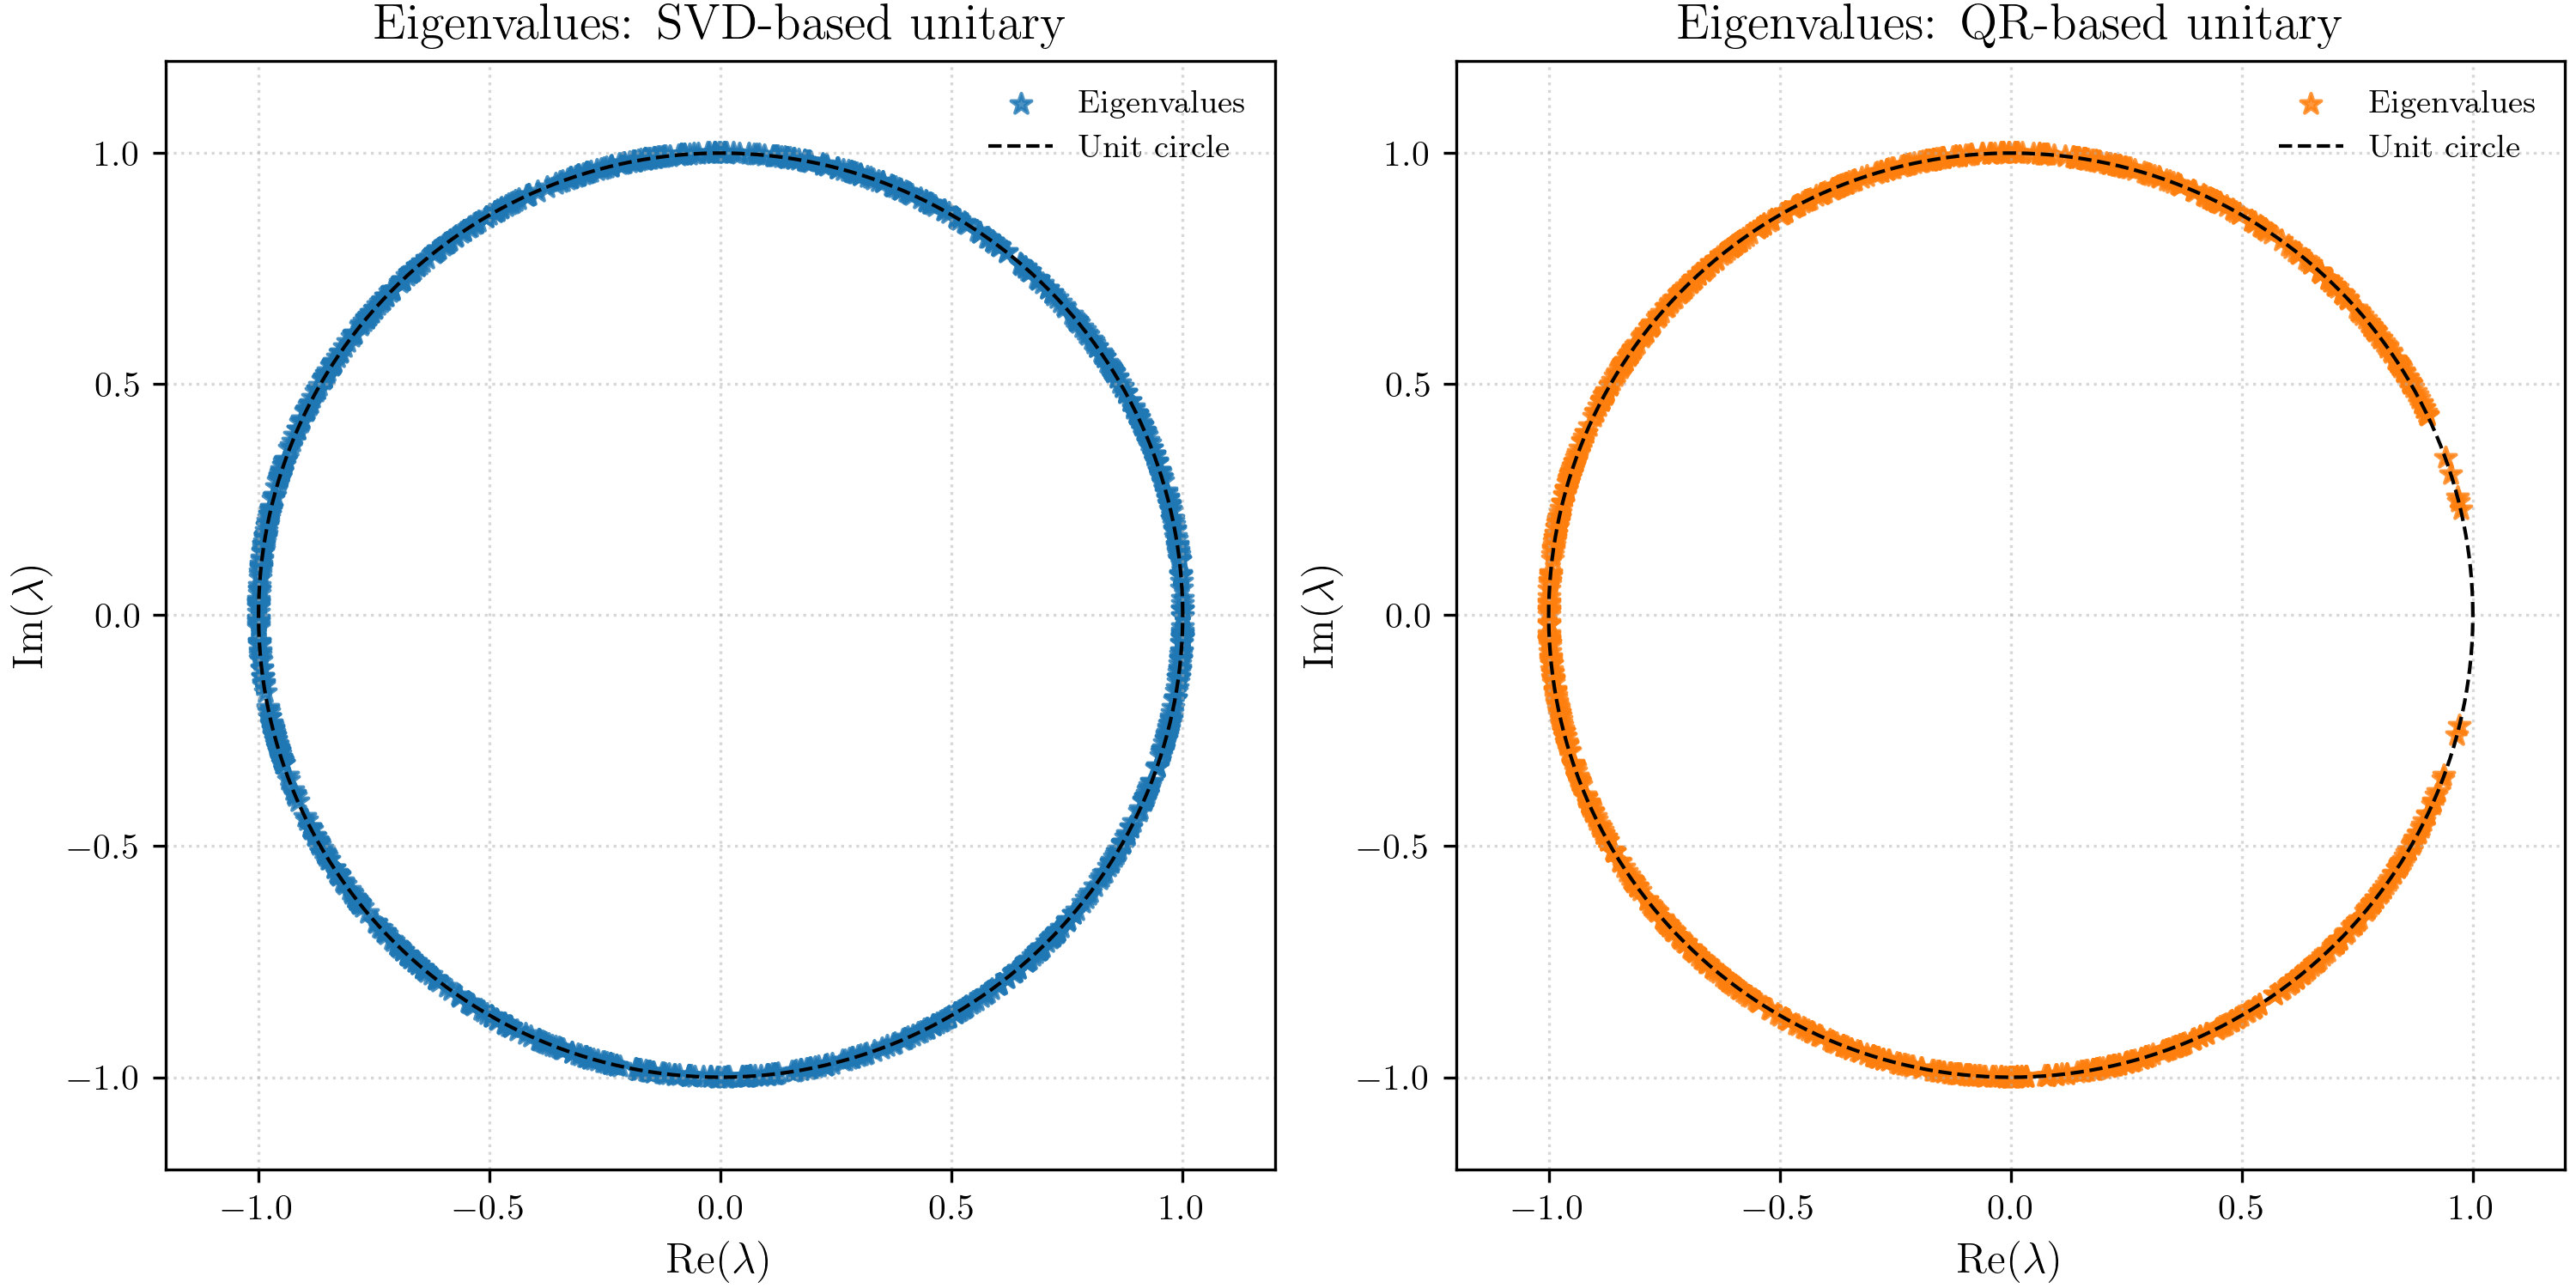
\includegraphics[width=1\textwidth]{Graphics/eigenvalue_comparison.png}
    \caption{Eigenvalue distributions of random unitary matrices generated via SVD and QR.}
    \label{fig:eigenvalue-comparison}
\end{figure}

\section{Spectral Density}

To get to the notion of the spectral density,
we will first need some more basic definitions to build on.
The reader is assumed to be familiar with the concepts of distributions.
Let us also recap that for $\Omega \subset \C^n$ open and non-empty,
a \emph{test function} is a smooth function with compact support defined on $\Omega$.
The space of all test functions on $\Omega$ is usually denoted by $\mathcal{E}$.

We will now look at an important case of a distribution

\begin{definition}[Dirac delta distribution]
    Let $\mathcal{E} = \Cinfty(\Omega)$ with $0 \in \Omega \subset \R^n$.
    Then
    $$\delta: \mathcal{E} \to \R, \quad f \mapsto f(0) \quad \text{with} \quad \delta(f) = \langle \delta, f \rangle = f(0)$$
\end{definition}

this distribution is often mistakenly referred to as a function,
although it is not a function in the classical sense.\\
The Dirac delta is characterized by the following property:

\[
\int\limits_{-\infty}^{\infty} f(x) \delta(x-a) \dx = \int\limits_{-\infty}^{\infty} f(x) \delta(a-x) \dx = f(a) \implies \int\limits_{-\infty}^{\infty} \delta(x-a) \dx = 1.
\]

This means that the Dirac delta distribution is zero everywhere except at the point $a$,
where it is infinitely high, such that the integral over it equals $1$.
We now have all the tools we need to define the central concept of this thesis:

\begin{definition}[Spectral density]
    Let $H$ be hermitian and sparse.
    For $x \in \R$, the \emph{spectral density} is then defined as
    \[
    \phi(x) = \frac{1}{n} \sum_{j=1}^{n} \delta(x - \lambda_j)
    \]
    where $\delta$ is the Dirac delta distribution
    and $\lambda_j$ are the eigenvalues of $H$ in non-descending order.
\end{definition}

The number of eigenvalues in an interval $[a, b]$ can then be counted in the following manner:

\begin{equation} \label{eq:nu_a_b}
    \nu_{[a, b]} = \int\limits_a^b \sum_j \delta(t - \lambda_j) \dt \equiv \int\limits_a^b n \phi(t) \dt
\end{equation}

Random matrix theory tells us that the eigenvalues of random unitary matrices are distributed uniformly on the unit circle.
Thus, we would expect the spectral density to be uniformly distributed on the unit circle as well.
This is important as we think of the choice of random unitary matrices.

If we generate a random complex square matrix $A$,
there are multiple ways to obtain a unitary matrix $U$.
We will now compare the svd with the qr decomposition.

Before we can proceed to the motice of this thesis, we will need to define the following space:

\begin{definition}[Schwartz space over $\R$] \label{def:Schwartz space}
    The \emph{Schwartz space} over $\R$ consists of all smooth functions $f$ that decay rapidly to zero as $|x|$ approaches infinity \cite{richtmyer}.
    Formally,
    \[
    \SR := \left\{f \in \Cinfty(\R) \mid \forall p, k \in \N_0: \sup_{x \in \R} \left| x^p f^{(k)}(x) \right| < \infty \right\}
    \]
\end{definition}

\chapter{Motivation}
\section{Motivation}
Calculating the spectral density of a matrix is trivial, when its eigenvalues are already known.
However, this is mostly not the case and calculating eigenvalues of very large matrices is time- and energy intensive.
At the same time, the DOS as a kind of probability density over the distribution of eigenvalues is of great interest in many fields.
Thus, there is a need for methods which approximate the spectral density at low cost.
The problem with this is that $\phi(t)$ the Delta distribution is not a \emph{function} as we know it,
that can be evaluated at each point.\\
A more intuitive idea would be to choose an intervall $I \in \R$ such that the spectrum of $A$, $\sigma(A)$, is a subset of $I$.
Now choose $k$ points $t_i$ in $I$, such that the intervall is divided in sub intervals:
$$\{t_i\}_{i = 1}^k \subset I \quad \text{mit} \quad \bigcup_{i = 1}^{k - 1} [t_i, t_{i+1}] = I$$
Now count the eigenvalues in every sub interval.
Then calculate the average value of $\phi(t)$ in every intervall with $\nu_{[a, b]}$ from equation \ref{eq:nu_a_b}.
The results is histograms, which with increasingly smaller subintervalls, that is to say bigger $k$ and $(t_{i+1} - t_i) \longrightarrow 0$, approach the spectral density.\\
To count the eigenvalues in the intervals, there is means like for example the Sylvestreschen Trägheitssatz.
The details of this method are not part of this work,
it would be necessary to calculate a decomposition of $A - t_i I = LDL^T$ for all $t_i$ \cite{golubvanloan}.
We prefer a method in which $A$ is multiplied with vectors, which is in bigger dimensions.\\
For simplicity we are going to assume, that $A$ is szmmetric and real.
The extension to hermetian matrices is simple in comparison.

\chapter{Kernel Polynomial Method}
\section{Overview}
There exists a whole class of methods, all of which called the kernel polynomial method, or KPM for short.
They are powerful tools for approximating the spectral density of matrices.
We will focus on the main approach in the following.\\
As the name suggests, the KPM is a polynomial extension of the spectral density.
The coefficients of the polynomials are derived from the method of moments,
in order to obtain an estimator function as in statistics.

The method is based on a corollary of the following generalized theorem:

\begin{theorem}
    Let $A \in \C^{n \times n}$ be a normal matrix with spectral decomposition
    \[
    A = U \Lambda U^* \quad \text{where} \quad UU^* = I_n \text{ and } \Lambda = \diag(\lambda_1, ..., \lambda_n)
    \]
    Let $\beta, v \in \C^n$ with $v = U\beta$.
    Suppose $v$ is a random vector whose entries $v_i$ are independent and identically distributed standard complex normal variables,
    i.e., $v_i \sim_\text{i.i.d.} \mathcal{N}_\C(0, 1)$, meaning $\Real(v_i), \Imag(v_i)$ are independent $\mathcal{N}(0, \frac{1}{2})$.
    Then
    \begin{equation} \label{eq:complex_normal_vector}
        \E[v] = 0 \quad \text{and} \quad \E[v v^*] = I_n,
    \end{equation}
    and it follows that
    \[
    \E[\beta] = 0 \quad \text{and} \quad \E[\beta \beta^*] = I_n.
    \]
\end{theorem}


\begin{proof}[Proof of Theorem 1]
    Since the expectation operator is linear, it holds that
    \[
    \E[v] = \E[U\beta] = U\E[\beta] = 0 \implies \E[\beta] = 0
    \]
    Furthermore it holds that
    \[
    I_n = \E[vv^*] = \E[(U\beta)(U\beta)^*] = \E[U\beta \beta^*U^*] = U \E[\beta \beta^*]U^*
    \]
    Multiplying both sides with $U^*$ and $U$ yields:
    \[
    U^* I_n U = U^* U \E[\beta \beta^*]U^* U = \E[\beta \beta^*]
    \]
    Since $U$ is unitary, we have shown that $\E[\beta \beta^*] = I_n$.
\end{proof}


\vspace{0.5 cm}
This theorem has a nice corollary when investigating a matrix function $f(A)$.
In that case, we have

\begin{align*}
    \E\left[v^* f(A) v\right] &= \E\left[(U\beta)^* f(U\Lambda U^*) (U\beta)\right] \\
        &= \E\left[\beta^* U^* U f(\Lambda) U^* U \beta\right] \\
        &= \E\left[\beta^* f(\Lambda) \beta\right] \\
        &= \E\left[\sum_{j = 1}^n |\beta_j|^2 f(\lambda_j) \right] \\
        &= \sum_{j = 1}^n f(\lambda_j) \E\left[ |\beta_j|^2 \right] \\
        &= \sum_{j = 1}^n f(\lambda_j)
\end{align*}

or, more concisely,
\begin{equation} \label{eq:theorem_result}
    \E\left[v^* f(A) v\right] = \Tr(f(A)).
\end{equation}

\section{Polynomial Extension with Chebyshev polynomials}
We assume Chebyshev polynomials to be a good fit for the polynomial extension of the Dirac delta distribution
because of the many great properties we will see now. First, let's look how Chebyshev polynomials are defined.
Using the trigonometric functions, they can be expressed as follows:

\[ T_k(x) =
\begin{cases}

\cos(k \arccos(x))                & \quad \text{for } k \in [-1, 1]\\
    \cosh(k \arcosh(x))           & \quad \text{for } k > 1\\
    (-1)^k \cosh(k \arcosh(-x))   & \quad \text{for } k < -1
\end{cases}
\]

We will only use the formula $T_k(x) = \cos(k \arccos(x))$.
This means to only consider matrices, which have eigenvalues within the intervall $[-1, 1]$.
In the case that this condition should not be fulfilled, the eigenvalues can be transformed accordingly.
For this, let $\lambda_{lb}$ and $\lambda_{ub}$ be the lower and upper bound for the eigenvalues of $A$, respectively.
To find these, well-established methods like the Gershgorin circle theorem can be used.

Define
\[
c := \frac{\lambda_{lb} + \lambda_{ub}}{2} \quad \text{and} \quad d := \frac{\lambda_{ub} - \lambda_{lb}}{2}
\]
Then, the matrix $B = \frac{A - c*I_n}{d}$ has eigenvalues in the interval $[-1, 1]$.
A visualization of this is linked in the appendix.


Another way to define Chebyshev polynomials is by calculating them using the recursion formula
\[
T_{k + 1}(x) = 2xT_k(x) - T_{k - 1}(x),
\]
where the starting conditions are given by $T_0(x) = 1$ and $T_1(x) = x$.

Additionally, note that the result in equation \ref{eq:theorem_result} says, that

\begin{equation} \label{eq:Chebyshev_trace}
    \E\left[\,v^T T_k(A) v\,\right] = \Tr\left(T_k(A)\right).
\end{equation}

This result will be central in the following discussion.


Now, let
\begin{equation} \label{eq:weight_function}
    h(x) = \frac{1}{\sqrt{1 - x^2}}
\end{equation}
be a weight function.
Another property of Chebyshev polynomials is
that they are \emph{orthogonal} in terms of the scalar product weighted with $h$:

\[
\left \langle f, g \right \rangle = \int_{-1}^1 \frac{1}{\sqrt{1 - x^2}} \cdot f(x) \cdot g(x) \dx.
\]

This means that

\[
\int_{-1}^1 \frac{1}{\sqrt{1 - t^2}} \cdot T_k(t) \cdot T_l(t) \dt =
\begin{cases}
    0               & \quad \text{for } k \neq l\\
    \pi             & \quad \text{for } k = l = 0\\
    \frac{\pi}{2}   & \quad \text{for } k = l \neq 0
\end{cases}
\]

\section{Approximating the spectral density}
Now multiply the spectral density with the inverse of the weight function \ref{eq:weight_function}:
\[
\hat{\phi}(x) = \sqrt{1 - x^2} \phi(x) = \sqrt{1 - x^2} \, \cdot \, \frac{1}{n} \sum_{j = 1}^n \delta(x - \lambda_j)
\]
Let $g \in \SR$, the Schwartz space defined in definition \ref{def:Schwartz space},
and $\mu_k \in \R$ coefficients to be determined such that the following equation holds:

\begin{equation} \label{eq:distribution_equality}
    \int \limits_{-1}^1 \hat{\phi}(t) g(t) \dt = \int \limits_{-1}^1 \sum_{k = 0}^{\infty} \mu_k T_k(t) g(t) \dt
\end{equation}

If this is true for arbitrary $g \in \SR$, we can simplify our equation \ref{eq:distribution_equality} to

\begin{equation} \label{eq:Chebyshev-Expansion}
    \hat{\phi}(x) = \sum_{k = 0}^{\infty} \mu_k T_k(x)
\end{equation}


Now utilize the orthogonality of the Chebyshev polynomials, to calculate a specific coefficient $\mu_k$:

\begin{align*}
    & \; \; \sum_{l = 0}^{\infty} \mu_l T_l(t) = \hat{\phi}(t) \\
    \implies & \left(\sum_{l = 0}^{\infty} \mu_l T_l(t)\right) \cdot T_k(t) = \hat{\phi}(t) \cdot T_k(t)\\
    \implies & \int_{-1}^1 \frac{1}{\sqrt{1 - t^2}} \cdot \left(\sum_{l = 0}^{\infty} \mu_l T_l(t)\right) \cdot T_k(t) \dt = \int_{-1}^1 \frac{1}{\sqrt{1 - t^2}} \cdot \hat{\phi}(t) \cdot T_k(t) \dt\\
    \implies & \mu_k \cdot \frac{\pi}{2 - \delta_{k0}} = \int_{-1}^1 \frac{1}{\sqrt{1 - t^2}} \cdot \sqrt{1 - t^2} \cdot \phi(t) \cdot T_k(t) \dt\\
    \implies & \mu_k = \frac{2 - \delta_{k0}}{\pi} \cdot \int_{-1}^1 \phi(t) \cdot T_k(t) \dt\\
\end{align*}

By applying the Dirac delta distribution we obtain:
\begin{align*}
    \mu_k = \frac{2 - \delta_{k0}}{\pi} \cdot \int_{-1}^1 \phi(t) \cdot T_k(t) \dt &= \frac{2 - \delta_{k0}}{\pi} \cdot \int_{-1}^1 \frac{1}{n} \sum_{j = 1}^n \delta(t - \lambda_j) \cdot T_k(t) \dt \\
    &= \frac{2 - \delta_{k0}}{n \pi} \sum_{j = 1}^n T_k(\lambda_j)\\
    &= \frac{2 - \delta_{k0}}{n \pi} \Tr(T_k(A))
\end{align*}

Now let $n_{\text{vec}} \in \R$ and consider vectors $v_0^{(1)}, v_0^{(2)}, \dots, v_0^{(n_{\text{vec}})}$,
which are chosen randomly from the standard normal distribution,
that is to say $\E[v_0^{(k)}] = 0$ und $\E\left[v_0^{(k)}\left(v_0^{(k)}\right)^T\right] = I_n$.
It follows from equation \ref{eq:Chebyshev_trace} that
\[
\zeta_k = \frac{1}{n_{\text{vec}}} \sum_{l = 1}^{n_{\text{vec}}} \left( v_0^{(l)} \right)^T T_k(A) v_0^{(l)}
\]
is a good estimator for $\Tr(T_k(A))$ and therefore
\[
\mu_k \approx \frac{2 - \delta_{k0}}{n \pi} \zeta_k
\]

In order to determine the $\zeta_k$, let $v_0 \equiv v_0^{(l)}$
Using the recursion formula for Tschebyschev polynomials, we can calculate
\[
T_{k + 1}(A)v_0 = 2 A T_k(A) v_0 - T_{k - 1}(A) v_0
\]
For $v_k \equiv T_k(A)v_0$ it also holds that
\[
v_{k + 1} = 2 A v_k - v_{k - 1}
\]

With this we are fully equpped for the final calculation and the goal of the KPM is reached:
Instead of having to multiply matrices with other matrices, it now suffices to multiply matrices with vectors.
Now we can approximate $\phi(x)$ as closely as we like.
As aforementioned, it is not always desirable to have an infinitely exact approximation.
Since it holds that
\[
\lim \limits_{k \to \infty} \mu_k \to 0
\]
and we are only interested in $T_k(x)$ with $k \leq M$\\
Therefore we estimate $\phi$ with
\begin{equation} \label{eq:Angenäherte Spektraldichte}
    \tilde{\phi}_M(x) = \frac{1}{\sqrt{1 - x^2}} \sum_{k = 0}^{M} \mu_k T_k(x)
\end{equation}

The following pseudo code is based on \cite[p.~10]{linsaadyang14} and summarizes the steps described above.
The implementation is done in Python, and linked in the appendix.

\begin{algorithm}
    \caption{The Kernel Polynomial Method}\label{alg:cap}
    \begin{algorithmic}[5]
    \Require $A = A^* \in \mathbb{C}^{n \times n}$ with eigenvalues in the intervall $[-1, 1]$
    \Ensure Estimated spectral density \{$\tilde{\phi}_M(t_i)$\}\\
    \For{$k = 0 : M$}
    \State $\zeta_k \gets 0$
    \EndFor
    \For{$l = 1 : n_{\text{vec}}$}
    \State $\text{Choose a random new vector } v_0^{(l)}\text{;}$ \Comment{$v_{0_i}^{(l)} \sim_\text{ i.i.d. } \mathcal{N}(0, 1)$}
    \For{$k = 0 : M$}
    \State $\text{Calculate } \zeta_k \gets \zeta_k + \left( v_0^{(l)} \right)^T v_k{(l)}\text{;}$  
    \If{$k = 0$}
    \State $v_1^{(l)} \gets A v_0^{(l)}$
    \Else
    \State $v_{k+1}^{(l)} \gets 2 A v_k^{(l)} - v_{k-1}^{(l)}$ \Comment{Three term recursion}
    \EndIf
    \EndFor
    \EndFor
    \For{$k = 0 : M$}
    \State $\zeta_k \gets \frac{\zeta_k}{n_{\text{vec}}}$
    \State $\mu_k \gets \frac{2 - \delta_{k0}}{n \pi} \zeta_k$
    \EndFor
    \State $\text{Evaluate } \tilde{\phi}_M(t_i) \text{ with equation } \ref{eq:Angenäherte Spektraldichte}$
    \end{algorithmic}
\end{algorithm}

Applying the Cayley transform to an arbitrary unitary matrix $U$ yields a Hermitian matrix $H$;
and as this is the case, the KPM can be applied to unitary matrices as well.

\chapter{Quality Analysis}
Let $\tilde{\phi}(t)$ be a regular function, that estimates the spectral density.
Since $\phi(t)$ is no function in the classical sense, but all approximations are continuous functions,
\[
\left|\left|\phi(t) - \tilde{\phi}(t)\right|\right|_{L^p}
\]
is not defined, to estimate the error.
In the following, we will introduce two methods to circumvent this problem.
The first one uses the fact that $\delta(t)$ is a distribution that can be applied to test functions from the Schwartz space $\SR$,
while the second one regularizes $\delta$-functions by replacing them with continuous and smooth functions.
These two approaches are closely related, as we will see later.

\section{Resolution}
In practice, there is often no need to approximate all eigenvalues of $A$ exactly.
This would even be highly discontinuous, as we recall the intuitive approach with histograms.
The accuracy of the approximation should be oriented towards the desired \emph{resolution}.
This means that often only the eigenvalues in a certain subinterval $[a, b] \subset \sigma(A)$ are of interest in a certain context.
The size $b - a$ is then called the resolution of the estimate.
This insight should be taken as a parameter in our further considerations.

\section{Restriction on the Schwartz space}
In this first method, we consider $\delta(t)$ as a distribution.
Let $g \in \Cinfty(\R)$ be a test function from the Schwartz space $\SR$ defined in Definition \ref{def:Schwartz space}.
Then we have
\[
\langle \delta(\cdot - \lambda), g \rangle = \int\limits_{-\infty}^{\infty} \delta(t - \lambda) g(t) \dt = g(\lambda)
\]
and for all $p, k \in \N_0$
\[
\sup_{t \in \R} |t^pg^{(k)}(t)| < \infty
\]
The error can therefore be measured as follows:
\[
\epsilon_1 = \sup_{g \in \SR} \left| \langle \phi, g \rangle - \langle \tilde{\phi}, g \rangle \right|
\]

To transfer the concept of resolution to this error,
we first consider $\nu_{[a, b]}$ from equation \ref{eq:nu_a_b} and define accordingly
\[
\tilde{\nu}_{[a, b]} = \int\limits_a^b n \tilde{\phi}(t) \dt
\]
with $\tilde{\phi}(t) \in \Cinfty(\R)$.
Assuming $n = 1$ and thus $\phi(t) = \delta(t)$,
an infinite resolution would mean that for arbitrarily small intervals $[a, b]$ the term $\left| \nu_{[a, b]} - \tilde{\nu}_{[a, b]} \right|$ also becomes arbitrarily small.
Let $a = -\varepsilon, b = \varepsilon$.
From the definition of the $\delta$-function it follows that
$$\lim \limits_{\varepsilon \to 0+} \nu_{[-\varepsilon, \varepsilon]} = 1$$
while for smooth functions $\tilde{\phi}$ it is clear that
$$\lim \limits_{\varepsilon \to 0+} \tilde{\nu}_{[-\varepsilon, \varepsilon]} = 0$$
This shows that no smooth function converges to the spectral density under continuous increase of the resolution.
A carefully balanced approximation would therefore be as precise as a constant one.
However, as noted earlier,
a finite resolution is often sufficient.
We can therefore restrict the Schwartz space $\SR$.
For example, one could only consider Gaussian distributions of the form
$$g_{\sigma}(t) = \frac{1}{(2\pi\sigma^2)^\frac{1}{2}}e^{-\frac{t^2}{2\sigma^2}}$$
and restrict $\SR$ to the subspace
$$\SR(\sigma;[\lambda_{us}, \lambda_{os}]) = \left\{ g \mid g(t) \equiv g_{\sigma}(t - \lambda), \lambda \in [\lambda_{us}, \lambda_{os}] \right\}$$
Here, $\lambda_{us}$ and $\lambda_{os}$ are the upper and lower bounds of the eigenvalues of $A$ as in the previous section,
while the parameter $\sigma$ represents the \emph{target resolution}.
We can now use the following metric for quality assessment:

\begin{equation} \label{eq:error}
    E\left[\tilde{\phi};\SR\left(\sigma; \left[\lambda_{lb}, \lambda_{ub} \right] \right)\right] = \sup_{g \in \SR(\sigma;[\lambda_{lb}, \lambda_{ub}])} \left| \langle \phi, g \rangle - \langle \tilde{\phi}, g \rangle \right|
\end{equation}

\section{Regularizing the Dirac delta distribution}
In the second method, we regularize the $\delta$-function.
This means that we replace the $\delta$-function with a smooth function $\phi(t)$
that approximates the spectral density.
This is done by smoothing the $\delta$-function.
For example, we can use the Gaussian distribution with standard deviation $\sigma$:
$$\phi_{\sigma}(t) = \frac{1}{(2\pi\sigma^2)^\frac{1}{2}}e^{-\frac{t^2}{2\sigma^2}}$$
This function is smooth and well-defined for all $t \in \R$.
It is also normalized, meaning that
$$\int\limits_{-\infty}^{\infty} \phi_{\sigma}(t) \dt = 1$$
This means that $\phi_{\sigma}(t)$ can be interpreted as a probability density function.
The parameter $\sigma$ controls the width of the Gaussian distribution
and thus the resolution of the approximation.
This means that the smaller $\sigma$ is, the more precise the approximation is,
but also the more sensitive it is to noise in the data.
This is a common approach in numerical analysis to approximate distributions with smooth functions.
The function $\phi_{\sigma}(t)$ is then well-defined and can be used to calculate the error for $p=1, 2$ and $\infty$:
\[
\epsilon_2 = \left|\left| \phi_{\sigma}(t) - \tilde{\phi}(t) \right|\right|_p
\]

Let
\[
\phi_{\sigma}(t) = \left \langle \phi(\cdot), g_{\sigma}(\cdot - t)\right \rangle = \sum_{j = 1}^n g_{\sigma}(t - \lambda_j)
\]
This is the convolution of the spectral density with the Gaussian function $g_{\sigma}$.
In similar manner, let
\[
\tilde{\phi}_{\sigma}(t) = \langle \tilde{\phi}(\cdot), g_{\sigma}(\cdot - t) \rangle
\]
Then
\[
E\left[\tilde{\phi};\SR\left(\sigma; \left[\lambda_{lb}, \lambda_{ub} \right] \right)\right] = \sup_{g \in \SR(\sigma;[\lambda_{lb}, \lambda_{ub}])} \left| \phi_{\sigma}(t) - \tilde{\phi}_{\sigma}(t) \right|
\]
is the $L^\infty$ error between two well-defined functions.
Just like in the other method, $\sigma$ controls the resolution:
the larger the $\sigma$, the smoother but also less accurate the approximation.
For smaller values, one obtains coarser functions,
where small peaks can be detected exactly where the eigenvalues are located.
The following graphic is taken from \cite[p.~6]{linsaadyang14} and illustrates this effect for four different values of $\sigma$:
Sei also
$$\phi_{\sigma}(t) = \left \langle \phi(\cdot), g_{\sigma}(\cdot - t)\right \rangle = \sum_{j = 1}^n g_{\sigma}(t - \lambda_j)$$
Dies ist dann nicht anderes als die "Weichzeichnung" der Spektraldichte durch Gauß-Funktionen der Breite $\sigma$.

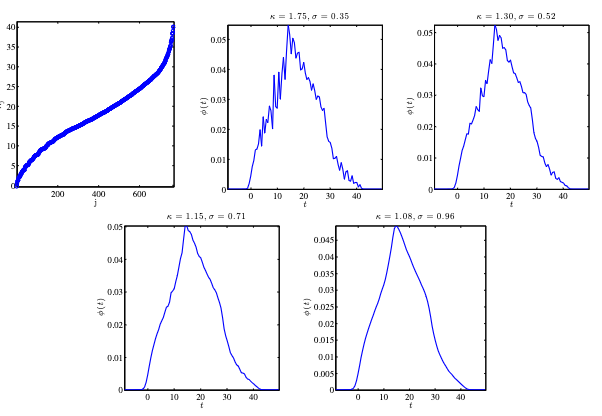
\includegraphics[height=7.5cm]{./Graphics/screenshot.png}

\section{The condition of non-negativity}
As a probability distribution, the spectral density is non-negative, meaning
\[
\forall g \in \SR, g \geq 0: \langle \phi, g \rangle \geq 0
\]
Some numerical approximations break this property, including the Kernel Polynomial Method.
This leads to large errors and must be considered carefully.
Methods to mitigate these negative effects would exceed the scope of this work.

\bibliographystyle{plain}
\begin{thebibliography}{56}

    \bibitem{baer18}
    \textsc{C. Bär},
    \textit{Lineare Algebra und analytische Geometrie},
    Springer Spektrum
    2018.

    \bibitem{golub2013matrix}
    \textsc{G. H. Golub and C. F. Van Loan},
    \textit{Matrix Computations},
    4th edition,
    Johns Hopkins University Press,
    Baltimore, MD,
    2013.

    \bibitem{sheldonaxler}
    \textsc{S. Axler},
    \textit{Linear Algebra Done Right},
    Springer,
    2015.

    \bibitem{higham}
    \textsc{N. J. Higham},
    \textit{Functions of Matrices: Theory and Computation},
    SIAM,
    2008.

    \bibitem{strichartz}
    \textsc{R. S. Strichartz},
    \textit{A Guide to Distribution Theory and Fourier Transforms},
    World Scientific,
    2003.

    \bibitem{reichl}
    \textsc{L. E. Reichl},
    \textit{A Modern Course in Statistical Physics},
    4th edition,
    Wiley-VCH,
    2016.

    \bibitem{sakurainapolitano}
    \textsc{J. J. Sakurai and J. Napolitano},
    \textit{Modern Quantum Mechanics},
    2nd edition,
    Addison-Wesley,
    2011.

    \bibitem{oppenheimschafer}
    \textsc{A. V. Oppenheim and R. W. Schafer},
    \textit{Discrete-Time Signal Processing},
    3rd edition,
    Prentice Hall,
    2010.

    \bibitem{mitra}
    \textsc{S. K. Mitra},
    \textit{Digital Signal Processing: A Computer-Based Approach},
    2nd edition,
    McGraw-Hill Science Engineering Math,
    2001.

    \bibitem{nortonkarczub}
    \textsc{M. P. Norton, D. G. Karczub},
    \textit{Fundamentals of Noise and Vibration Analysis for Engineers},
    Cambridge University Press,
    2003.

    \bibitem{mezzadri2007}
    \textsc{F. Mezzadri},
    \textit{How to generate random matrices from the classical compact groups},
    Notices of the AMS, 54(5), 592--604, 2007.
    doi:10.1090/noti209

    \bibitem{andersonguionnetzeitouni}
    \textsc{G. W. Anderson, A. Guionnet, O. Zeitouni},
    \textit{An Introduction to Random Matrices},
    Cambridge University Press,
    2010.

    \bibitem{weisse2006}
    \textsc{A. Weisse, G. Wellein, A. Alvermann, H. Fehske},
    \textit{The kernel polynomial method},
    Reviews of Modern Physics, 78(1): 275--306, 2006.
    doi:10.1103/RevModPhys.78.275

    \bibitem{linsaadyang14}
    \textsc{L. Lin, Y. Saad, C. Yang},
    \textit{Approximating Spectral Densities of Large Matrices},
    SIAM Review, 58(1): 34--65, 2016.
    doi:10.1137/130933381

    \bibitem{richtmyer}
    \textsc{R. D. Richtmyer},
    \textit{Principles of Advanced Mathematical Physics},
    vol 1, Springer Verlag,
    New York,
    1981.

    \bibitem{PasSh11}
    \textsc{L. Pastur, M. Shcherbina},
    \textit{Eigenvalue Distribution of Large Random Matrices},
    AMS,
    2011.

\end{thebibliography}
    
\end{document}